 \documentclass{beamer}[10]

\usepackage{graphicx}
\usepackage{xcolor}
\usepackage{tabto}
%\usepackage{beamerthemesplit}
\usepackage{tikz}
\usepackage{cancel}
\usepackage{verbatim}
\usepackage{fancybox}
\usepackage{enumerate}
\usepackage{amsmath,amssymb,amsthm,textcomp,mathtools}
\usepackage[super]{nth}
\usepackage[amssymb]{SIunits}
\usepackage{booktabs}
\usepackage{cancel}
\usepackage{bm}
\usepackage[utf8]{inputenc}
\usepackage{tabularx}
\usepackage{ragged2e}
\newcolumntype{Y}{ >{\RaggedRight\arraybackslash}X}
\usetikzlibrary{arrows,shapes}
\newcommand\T{\rule{0pt}{2.6ex}}
\newcommand\B{\rule[-1.2ex]{0pt}{0pt}}
\definecolor{UUcrimson}{RGB}{204,0,0}
\mode<presentation>
{ \usetheme{default}
  \usecolortheme[named=UUcrimson]{structure}
  \useinnertheme{circles}
  \setbeamercovered{transparent}
  \setbeamertemplate{blocks}[rounded]
  \usefonttheme[onlymath]{serif}
  \setbeamertemplate{navigation symbols}{}
  \setbeamertemplate{footline}[page number]
  \setbeamertemplate{navigation symbols}{}
  \setbeamercolor{section in toc}{fg=black,bg=white}
  \setbeamercolor{alerted text}{fg=UUcrimson!80!gray}
  \setbeamercolor*{palette primary}{fg=white,bg=UUcrimson}
  \setbeamercolor*{palette secondary}{fg=UUcrimson!70!black,bg=gray!15!white}
  \setbeamercolor*{palette tertiary}{bg=UUcrimson!80!black,fg=gray!10!white}
  \setbeamercolor*{palette quaternary}{fg=UUcrimson,bg=gray!5!white}
  \setbeamercolor*{palette sidebar primary}{fg=UUcrimson!10!black}
  \setbeamercolor*{palette sidebar secondary}{fg=white}
  \setbeamercolor*{palette sidebar tertiary}{fg=UUcrimson!50!black}
  \setbeamercolor*{palette sidebar quaternary}{fg=gray!10!white}
  \setbeamercolor{titlelike}{parent=palette primary,fg=white}
  \setbeamercolor{frametitle}{bg=UUcrimson}
  \setbeamercolor{frametitle right}{bg=UUcrimson}
  \setbeamercolor*{separation line}{}
  \setbeamercolor*{fine separation line}{}
}

\usetikzlibrary{backgrounds}
\makeatletter
\tikzstyle{every picture}+=[remember picture]
\tikzset{%
  fancy quotes/.style={
    text width=\fq@width pt,
    align=justify,
    inner sep=1em,
    anchor=north west,
    minimum width=\linewidth,
    font=\itshape
  },
  fancy quotes width/.initial={.8\linewidth},
  fancy quotes marks/.style={
    scale=8,
    text=white,
    inner sep=0pt,
  },
  fancy quotes opening/.style={
    fancy quotes marks,
  },
  fancy quotes closing/.style={
    fancy quotes marks,
  },
  fancy quotes background/.style={
    show background rectangle,
    inner frame xsep=0pt,
    background rectangle/.style={
      fill=gray!25,
      rounded corners,
    },
  }
}
\newenvironment{fancyquotes}[1][]{%
\noindent
\tikzpicture[fancy quotes background]
\node[fancy quotes opening,anchor=north west] (fq@ul) at (0,0) {``};
\tikz@scan@one@point\pgfutil@firstofone(fq@ul.east)
\pgfmathsetmacro{\fq@width}{\linewidth - 2*\pgf@x}
\node[fancy quotes,#1] (fq@txt) at (fq@ul.north west) \bgroup}
{\egroup;
\node[overlay,fancy quotes closing,anchor=east] at (fq@txt.south east) {''};
\endtikzpicture}
\makeatother

\usepackage{scalerel}[2014/03/10]
\usepackage{stackengine}
\usepackage{empheq}
\newcommand*\widefbox[1]{\fbox{\hspace{0.5em}#1\hspace{0.5em}}}

\newcommand\reallywidetilde[1]{\ThisStyle{%
  \setbox0=\hbox{$\SavedStyle#1$}%
  \stackengine{-.1\LMpt}{$\SavedStyle#1$}{%
    \stretchto{\scaleto{\SavedStyle\mkern.2mu\sim}{.5467\wd0}}{.4\ht0}%
%    .2mu is the kern imbalance when clipping white space
%    .5467++++ is \ht/[kerned \wd] aspect ratio for \sim glyph
  }{O}{c}{F}{T}{S}%
}}
\usepackage{media9}

\logo{\includegraphics[width=0.75cm]{logo.jpg}}
\author[Gibbs]{Dr. Jeremy A. Gibbs}
\institute{Department of Mechanical Engineering\\University of Utah}
\date{Fall 2016}
\title{LES of Turbulent Flows: Lecture 21}
\begin{document}

%----------------------------------------------------------------------------------------
%	TITLE & TOC SLIDES
%----------------------------------------------------------------------------------------

\begin{frame} 
  \titlepage
\end{frame}

%------------------------------------------------

\begin{frame}
\frametitle{Overview}
\tableofcontents
\end{frame}

%------------------------------------------------
\section{Boundary Conditions for LES} %
%------------------------------------------------
\begin{frame}{Boundary Conditions for LES}
\begin{itemize}
	\item Like all numerical techniques for PDEs, LES requires the specification of boundary conditions
	\item Lateral or inflow/outflow conditions
	\item Boundary conditions at solid walls (particularly interesting for LES)
	\item Initial conditions (for time integration) can also be an important issue for some flows (\textit{e.g.}, decaying isotropic turbulence)
\end{itemize}
\end{frame}
%------------------------------------------------
\begin{frame}{Boundary Conditions for LES}
\begin{itemize}
	\item Note: in some flows, the top (upper) boundary conditions are also important
	\item One common example is of the ABL when buoyancy effects are present resulting in gravity waves
	\item The two most common ways of dealing with this are \underline{Rayleigh dampening}, where a sponge layer of points is defined, and \underline{linear wave canceling} (Klemp and Durran 1983)
\end{itemize}
\end{frame}
%------------------------------------------------
\begin{frame}{Boundary Conditions for LES}
\begin{itemize}
	\item We will talk about inflow boundary conditions, open (exit) boundary conditions, and boundary conditions at solid boundaries.  
	\item Today we will focus on inflow conditions (others to come in future lectures)
\end{itemize}
\end{frame}
%------------------------------------------------
\section{Inflow Boundary Conditions}
%------------------------------------------------
\begin{frame}{Inflow Boundary Conditions}
\begin{itemize}
	\item Issues related to lateral (flow direction) BCs are not specific to LES
	\item In DNS, nearly identical issues are present
	\item In RANS (many times), this issue is not important since appropriate conditions based on mean fields are all that may be needed
\end{itemize}
\end{frame}
%------------------------------------------------
\begin{frame}{Inflow Boundary Conditions}
\begin{itemize}
	\item Simplest case: \textbf{Periodic BCs}
	\item The idea is that what leaves the domain is returned identically
	\item For true boundary-layer flow (that grows in the flow direction) or flows with complex geometry, \textbf{many times we can't use periodic BCs}
	\item The figure on the next slide illustrates the importance of proper inflow BCs in a turbulent flow
	\item We will cover a few ways to deal with this (see Sagaut Ch 10.3)
\end{itemize}
\end{frame}
%------------------------------------------------
\begin{frame}{Inflow Boundary Conditions}
\begin{figure}
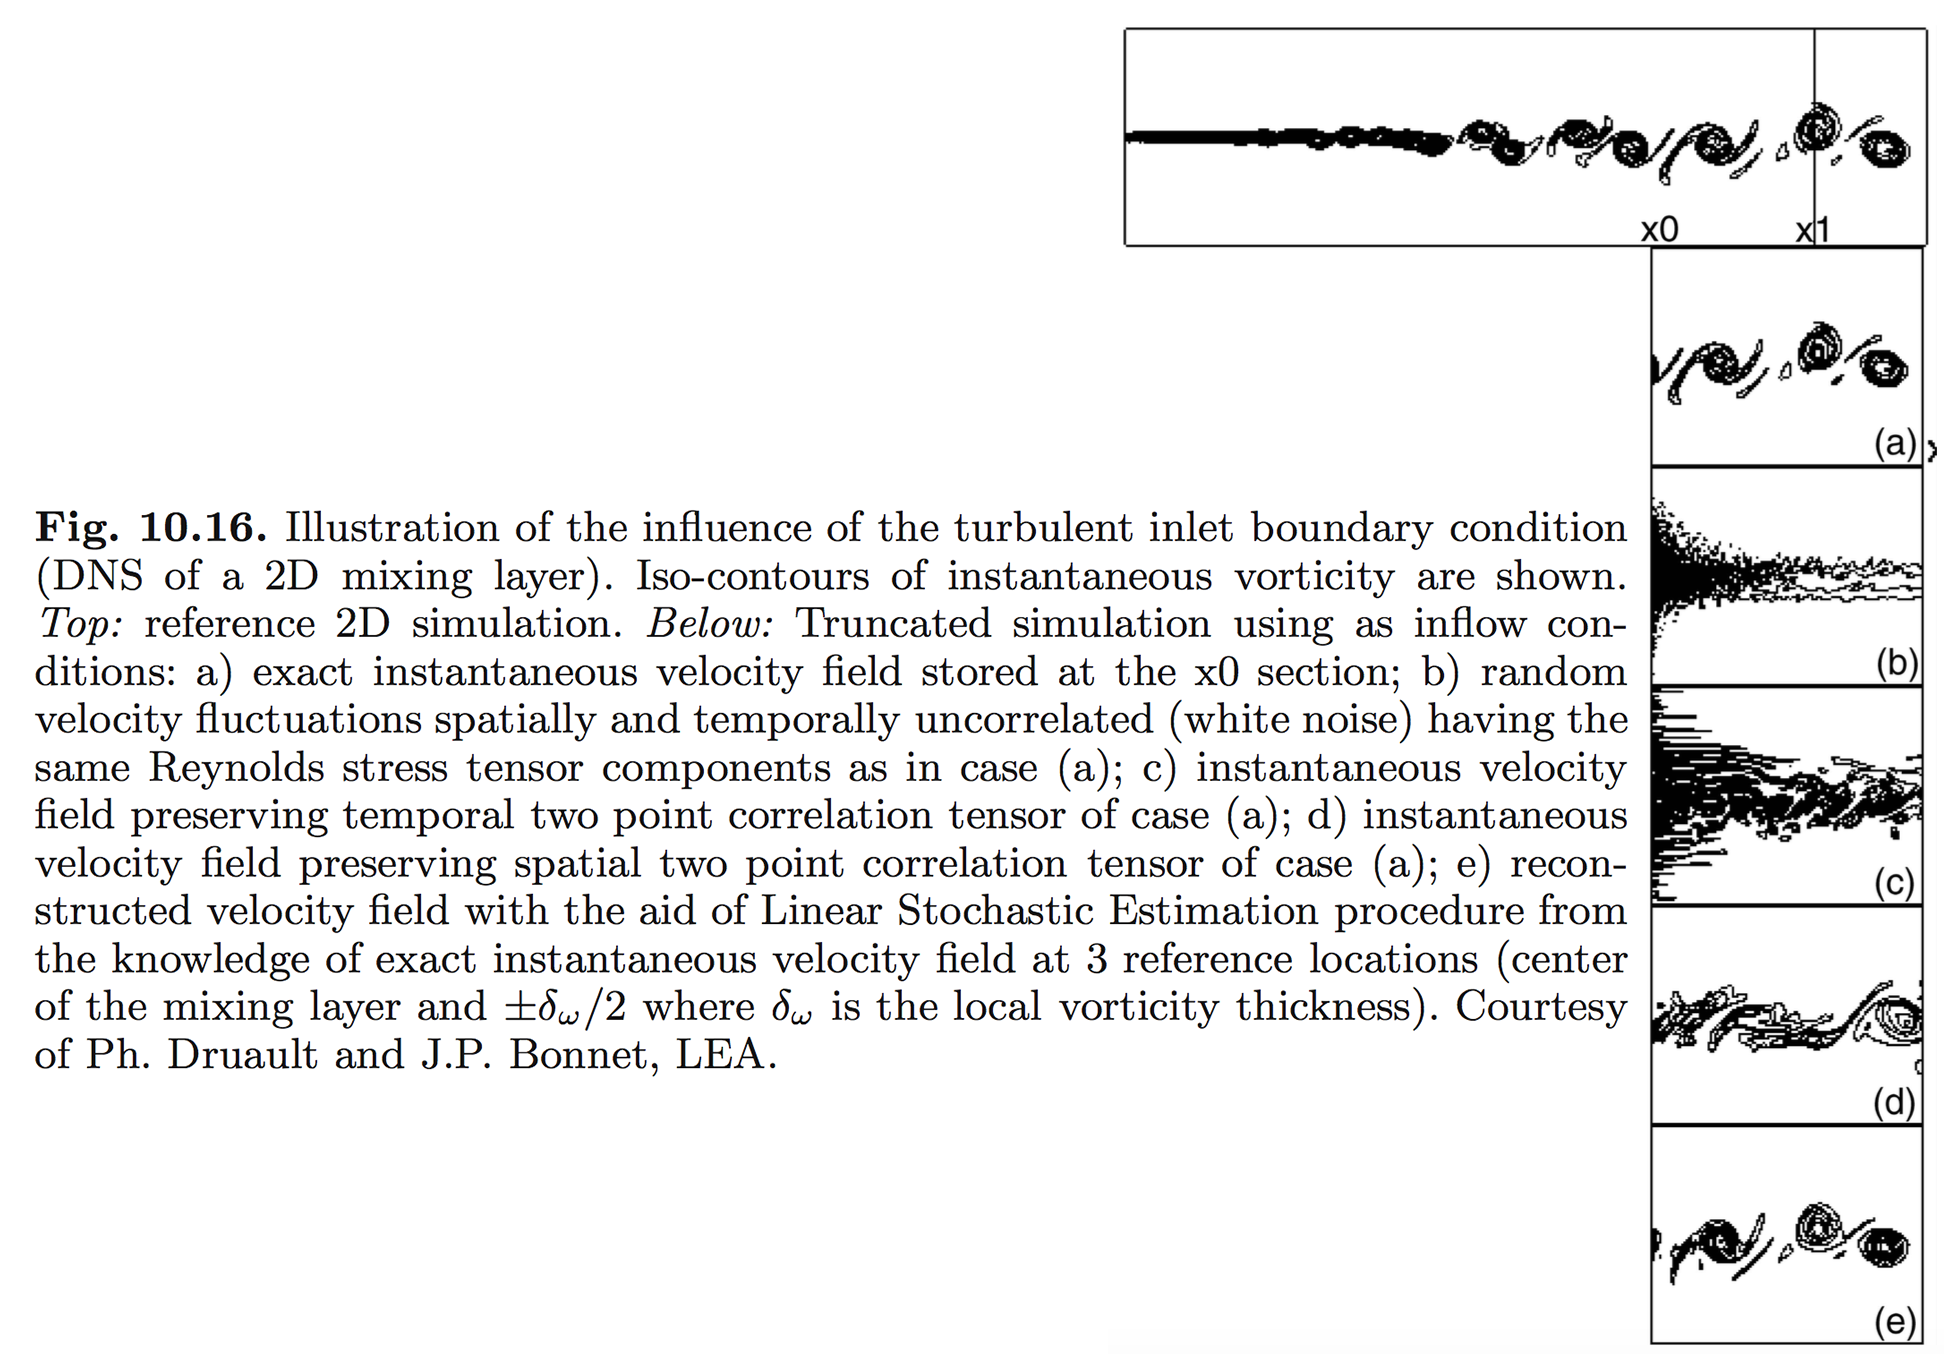
\includegraphics[height=0.8\textheight]{inlet1}
\end{figure}
\end{frame}
%------------------------------------------------
\begin{frame}{Inflow Boundary Conditions}
\begin{figure}
\includegraphics[width=0.55\textwidth]{inlet2}	
\end{figure}
Example from ME Ph.D. student Arash Nemati Hayati (in review)
\end{frame}
%------------------------------------------------
\begin{frame}{Inflow Boundary Conditions}
\centering
Courtesy Arash Nemati Hayati (requires Adobe)
\includemedia[
  width=0.7\textwidth,
  height=0.7\textwidth,
  activate=pageopen,
  addresource=inlet1.mp4,
  flashvars={source=inlet1.mp4}
]{}{VPlayer.swf}
\end{frame}
%------------------------------------------------
\begin{frame}{Inflow Boundary Conditions}
\centering
Courtesy Arash Nemati Hayati (requires Adobe)
\includemedia[
  width=0.7\textwidth,
  height=0.7\textwidth,
  activate=pageopen,
  addresource=inlet2.mp4,
  flashvars={source=inlet2.mp4}
]{}{VPlayer.swf}
\end{frame}

%------------------------------------------------
\subsection{Stochastic Recontruction}
%------------------------------------------------
\begin{frame}{Stochastic Recontruction}
	\begin{itemize}
	\item Deterministic information is lost when describing the flow statistically
	\item The idea is to generate instantaneous realizations that are statistically equivalent to the flow (\textit{i.e.}, same statistical moments)
	\item Most techniques try to specify boundary conditions by adding random noises (with same statistical moments as fluctuations) to the mean profile
	$$\tilde{u}(x_o,t) = \langle \tilde{u}(x_o)\rangle + u^\prime (x_o,t)$$ 
	\end{itemize}
\end{frame}
%------------------------------------------------
\begin{frame}{Stochastic Recontruction}
	\begin{itemize}
	\item Many of these techniques use an assumed energy spectrum combined with assumed BL profiles, or require other \textit{a priori} knowledge of turbulence statistics of the exact flow
	\item See Sagaut page 356 for a list of these methods
	\item While energy levels and 1-pt correlations (Reynolds stresses) info is retained, 2-pt space-time correlations are not reproduced
	\item That means phase information is lost, which can be important for shear flows (jet, mixing layer, BL) where consistency of fluctuations is important 
	\end{itemize}
\end{frame}
%------------------------------------------------
\begin{frame}{Stochastic Recontruction}
	\begin{itemize}
	\item What does this mean practically?
	\item There is a region in the computational domain where the flow has to regenerate the space-time consistency (a spin-up zone)
	\item The data here is useless and the zone can be large
	\item The scale of the zone is not known \textit{a priori}, which makes locating a place of interest within the domain very hard
	\end{itemize}
\end{frame}
%------------------------------------------------
\begin{frame}{Stochastic Recontruction}
	\begin{figure}
		\includegraphics[width=0.8\textwidth]{inlet6}
	\end{figure}
	\begin{itemize}
	\item An example from the WRF model. Imagine a standalone domain or a nested domain within a larger domain. This is how boundaries are defined.
	\end{itemize}
\end{frame}
%------------------------------------------------
\begin{frame}{Stochastic Recontruction}
\begin{figure}
\includegraphics[width=0.8\textwidth]{inlet5}	
\end{figure}
Example: LES grid nested within a large-scale WRF model run. Notice the large spin-up zone and small turbulence region.
\end{frame}
%------------------------------------------------
\subsection{Precursor Simulations Inflow Conditions}
%------------------------------------------------
\begin{frame}{Precursor Simulations Inflow Conditions}
	\begin{itemize}
	\item One of the most effective ways to generate inflow conditions is to specify inflow from ``homogeneous'' (\textit{e.g.}, horizontally homogeneous where we can use periodic conditions) pre-run flow simulations
	\item The idea is to perform a simulation of the upstream flow, called a \textit{precursor simulation}, with a degree of resolution equivalent to that desired for the final simulation
	\end{itemize}
\end{frame}
%------------------------------------------------
\begin{frame}{Precursor Simulations Inflow Conditions}
	\begin{figure}
		\includegraphics[width=0.8\textwidth]{inlet3}
	\end{figure}
	\begin{itemize}
	\item From Sagaut page 362: A precursor simulation of an attached boundary layer flow is performed. An extraction plane is defined, whose data are used as an inlet boundary condition for a simulation of the flow past a trailing edge
	\end{itemize}
\end{frame}
%------------------------------------------------
\begin{frame}{Precursor Simulations Inflow Conditions}
	\begin{figure}
		\includegraphics[width=0.75\textwidth]{inlet3}
	\end{figure}
	\textbf{Pros}:
	\begin{itemize}
	\item Requires very few assumptions
	\item We don't need an ``adjustment'' zone (as many other techniques do)
	\end{itemize}
\end{frame}
%------------------------------------------------
\begin{frame}{Precursor Simulations Inflow Conditions}
	\begin{figure}
		\includegraphics[width=0.75\textwidth]{inlet3}
	\end{figure}
	\textbf{Cons}:
	\begin{itemize}
	\item  Precursor simulations can be expensive (sometimes as much as the actual simulation of interest!) and they require large data storage and I/O. 
	\item The cost is sometimes decreased through interpolation in time between different precursor time steps
	\item There is no feedback of information from the \nth{2} simulation since the precursor is computed separately (\textit{i.e.} 1-way feedback)
	\end{itemize}
\end{frame}
%------------------------------------------------
\begin{frame}{Precursor Simulations Inflow Conditions}
	\begin{figure}
		\includegraphics[width=0.75\textwidth]{inlet3}
	\end{figure}
	\textbf{Cons}:
	\begin{itemize}
	\item There is no feedback of information from the \nth{2} simulation since the precursor is computed separately (\textit{i.e.} 1-way feedback)
	\item This can be an issue when a signal (\textit{e.g.}, acoustic wave) is emitted by the \nth{2}
	\end{itemize}
\end{frame}
%------------------------------------------------
\subsection{Rescaling}
%------------------------------------------------
\begin{frame}{Rescaling}
	\begin{figure}
		\includegraphics[width=0.6\textwidth]{inlet4}
	\end{figure}
	\begin{itemize}
	\item The flow from a downstream location, separated from the inflow enough to be considered independent is scaled (using known flow properties) to become the new inflow. Avoids need for precursor simulations	
	\end{itemize}
\end{frame}
%------------------------------------------------
\begin{frame}{Rescaling}
	\begin{figure}
		\includegraphics[width=0.6\textwidth]{inlet4}
	\end{figure}
	\begin{itemize}
	\item The flow at the extraction plane must be rescaled before being used at the inlet plane because the mean flow is not parallel (\textit{i.e.}, the BL thickness grows)
	\end{itemize}
\end{frame}
%------------------------------------------------
\begin{frame}{Rescaling}
Lund et al. (1998) algorithm
	\begin{itemize}
	\item Separate extracted flow into mean and fluctuating parts
	$$u_i^e (\vec{x},t) = U_i^e(y,z) + u_i^{\prime e} (\vec{x},t)$$
	\item The mean component classical scalings related to the mean velocity profile of the turbulent boundary layer (see Sagaut Sect 10.2.1)
	\item Law of the wall
	$$U^{\text{inner}} = u_\tau (x) f_1(z^+)\quad \text{where} \quad z^+ = \frac{z u_\tau}{\nu}$$
	\item Velocity defect law
	$$U_{\infty} - U^{\text{outer}} = u_\tau (x)f_2(\eta) \quad \text{where} \quad \eta = \frac{z}{\delta}$$
	\end{itemize}
\end{frame}
%------------------------------------------------
\begin{frame}{Rescaling}
Lund et al. (1998) algorithm
	\begin{itemize}
	\item These dictate that the mean velocity at the inlet must be related to the outlet by
	$$U_{\text{inlet}}^{\text{inner}} = \gamma U_{\text{recycle}}(y^+_{\text{inlet}})$$
	and
	$$U_{\text{inlet}}^{\text{outer}} = \gamma U_{\text{recycle}}(\eta_{\text{inlet}}) + (1-\gamma)U_{\infty}$$
	where
	$$\gamma = \frac{u_{\tau, \text{inlet}}}{u_{\tau, \text{recycle}}}$$
	\item From this, the mean velocity can be rescaled by interpolating the mean velocity at the recycle point to the same (non dimensional) height at the inlet
	\end{itemize}
\end{frame}
%------------------------------------------------
\begin{frame}{Rescaling}
Lund et al. (1998) algorithm
	\begin{itemize}
	\item Vertical velocity and fluctuating velocity are rescaled in a similar manner using empirical/theoretical functions
	\item These are then combined using
	\begin{align*}
	(u_i)_{\text{inlet}} &= \left[ (U_i)_{\text{inlet}^{\text{inner}}} + (u_i^\prime)_{\text{inlet}^{\text{inner}}}\right]\left[1 - W(\eta_\text{inlet})\right]\\
	&+ \left[ (U_i)_{\text{inlet}^{\text{outer}}}+ (u_i^\prime)_{\text{inlet}^{\text{outer}}}\right]W(\eta_\text{inlet})
	\end{align*}
	where $W$ is a weighting function that smoothly matches the profiles (tanh chosen by Lund et al 1998)
	\end{itemize}
\end{frame}
%------------------------------------------------
\begin{frame}{Rescaling}
\textbf{Caveats}:
	\begin{itemize}
	\item Very efficient in practice, but must be used carefully
	\item The recycling plane must be far enough from the inlet to prevent spurious couplings in the computed solution -- satisfied by taking a distance larger than the correlation length of the fluctuations in the streamwise direction
	\item Method is only valid for fully turbulent self-similar boundary layers
	\item Scaling laws must hold
	\end{itemize}
\end{frame}
%------------------------------------------------
\subsection{Synthetic Field Generation}
%------------------------------------------------
\begin{frame}{Synthetic Field Generation}
	Features of turbulence we seek to match synthetically
	\begin{itemize}
	\item Spatial correlation
	\item Temporal correlation
	\item Coherent across a broad range of scales
	\end{itemize}
	Random noise
	\begin{itemize}
	\item see examples above, this method tends to fail as a result of unrealistic velocity fields
	\end{itemize}
\end{frame}
%------------------------------------------------
\begin{frame}{Synthetic Field Generation}
	Fourier Based Methods
	\begin{itemize}
	\item General idea is to use Fourier expansion to specify the velocity field fluctuations
	\item Main advantage: spatial correlations are automatically preserved/included by use of continuous basis (sine/cosine) functions
	\item In general, assume (1D)
	$$u_x(y,t) = U_x(y) + u^\prime(y,t) = U_x(y) + D_{\text{norm}} \sum^N_{i=1} a_i^\prime (t) \cos(iky+\phi^\prime(t))$$
	where $D_{\text{norm}}$ is a scaling factor for the domain and discretization ($1/N$ for a domain of extent 1), $a_i^\prime$ are the Fourier coefficients, and $\phi^\prime$ are phase shift coefficients that can be used to control time correlations
	\end{itemize}
\end{frame}
%------------------------------------------------
\begin{frame}{Synthetic Field Generation}
	\begin{itemize}
	\item Other techniques include probability of detection (POD) and filtering-based methods
	\item Again, these are not as widely used to due to likelihood of failure due to unrealistic velocity fields
	\end{itemize}
\end{frame}
%------------------------------------------------

\end{document}

